\documentclass{beamer}[10]

\usepackage{graphicx}
\usepackage{xcolor}
\usepackage{tabto}
%\usepackage{beamerthemesplit}
\usepackage{tikz}
\usepackage{cancel}
\usepackage{verbatim}
\usepackage{fancybox}
\usepackage{enumerate}
\usepackage{amsmath,amssymb,amsthm,textcomp,mathtools}
\usepackage[super]{nth}
\usepackage[amssymb]{SIunits}
\usepackage{booktabs}
\usepackage{cancel}
\usepackage{bm}
\usepackage[utf8]{inputenc}
\usepackage{tabularx}
\usepackage{ragged2e}
\newcolumntype{Y}{ >{\RaggedRight\arraybackslash}X}
\usetikzlibrary{arrows,shapes}
\newcommand\T{\rule{0pt}{2.6ex}}
\newcommand\B{\rule[-1.2ex]{0pt}{0pt}}
\definecolor{UUcrimson}{RGB}{204,0,0}
\mode<presentation>
{ \usetheme{default}
  \usecolortheme[named=UUcrimson]{structure}
  \useinnertheme{circles}
  \setbeamercovered{transparent}
  \setbeamertemplate{blocks}[rounded]
  \usefonttheme[onlymath]{serif}
  \setbeamertemplate{navigation symbols}{}
  \setbeamertemplate{footline}[page number]
  \setbeamertemplate{navigation symbols}{}
  \setbeamercolor{section in toc}{fg=black,bg=white}
  \setbeamercolor{alerted text}{fg=UUcrimson!80!gray}
  \setbeamercolor*{palette primary}{fg=white,bg=UUcrimson}
  \setbeamercolor*{palette secondary}{fg=UUcrimson!70!black,bg=gray!15!white}
  \setbeamercolor*{palette tertiary}{bg=UUcrimson!80!black,fg=gray!10!white}
  \setbeamercolor*{palette quaternary}{fg=UUcrimson,bg=gray!5!white}
  \setbeamercolor*{palette sidebar primary}{fg=UUcrimson!10!black}
  \setbeamercolor*{palette sidebar secondary}{fg=white}
  \setbeamercolor*{palette sidebar tertiary}{fg=UUcrimson!50!black}
  \setbeamercolor*{palette sidebar quaternary}{fg=gray!10!white}
  \setbeamercolor{titlelike}{parent=palette primary,fg=white}
  \setbeamercolor{frametitle}{bg=UUcrimson}
  \setbeamercolor{frametitle right}{bg=UUcrimson}
  \setbeamercolor*{separation line}{}
  \setbeamercolor*{fine separation line}{}
}

\usetikzlibrary{backgrounds}
\makeatletter
\tikzstyle{every picture}+=[remember picture]
\tikzset{%
  fancy quotes/.style={
    text width=\fq@width pt,
    align=justify,
    inner sep=1em,
    anchor=north west,
    minimum width=\linewidth,
    font=\itshape
  },
  fancy quotes width/.initial={.8\linewidth},
  fancy quotes marks/.style={
    scale=8,
    text=white,
    inner sep=0pt,
  },
  fancy quotes opening/.style={
    fancy quotes marks,
  },
  fancy quotes closing/.style={
    fancy quotes marks,
  },
  fancy quotes background/.style={
    show background rectangle,
    inner frame xsep=0pt,
    background rectangle/.style={
      fill=gray!25,
      rounded corners,
    },
  }
}
\newenvironment{fancyquotes}[1][]{%
\noindent
\tikzpicture[fancy quotes background]
\node[fancy quotes opening,anchor=north west] (fq@ul) at (0,0) {``};
\tikz@scan@one@point\pgfutil@firstofone(fq@ul.east)
\pgfmathsetmacro{\fq@width}{\linewidth - 2*\pgf@x}
\node[fancy quotes,#1] (fq@txt) at (fq@ul.north west) \bgroup}
{\egroup;
\node[overlay,fancy quotes closing,anchor=east] at (fq@txt.south east) {''};
\endtikzpicture}
\makeatother


\usetikzlibrary{backgrounds}
\makeatletter
\tikzstyle{every picture}+=[remember picture]
\tikzset{%
  fancy defs/.style={
    text width=\fq@width pt,
    align=justify,
    inner sep=0.25em,
    anchor=north west,
    minimum width=\linewidth,
    font=\itshape
  },
  fancy defs width/.initial={.8\linewidth},
  fancy defs marks/.style={
    scale=8,
    text=white,
    inner sep=0pt,
  },
  fancy defs opening/.style={
    fancy defs marks,
  },
  fancy defs closing/.style={
    fancy defs marks,
  },
  fancy defs background/.style={
    show background rectangle,
    inner frame xsep=0pt,
    background rectangle/.style={
      fill=gray!25,
      rounded corners,
    },
  }
}
\newenvironment{fancydefs}[1][]{%
\noindent
\tikzpicture[fancy defs background]
\node[fancy defs opening,anchor=north west] (fq@ul) at (0,0) {};
\tikz@scan@one@point\pgfutil@firstofone(fq@ul.east)
\pgfmathsetmacro{\fq@width}{\linewidth - 2*\pgf@x}
\node[fancy defs,#1] (fq@txt) at (fq@ul.north west) \bgroup}
{\egroup;
\node[overlay,fancy defs closing,anchor=east] at (fq@txt.south east) {};
\endtikzpicture}
\makeatother
\usepackage{scalerel}[2014/03/10]
\usepackage{stackengine}
\usepackage{empheq}
\newcommand*\widefbox[1]{\fbox{\hspace{0.5em}#1\hspace{0.5em}}}

\newcommand\reallywidetilde[1]{\ThisStyle{%
  \setbox0=\hbox{$\SavedStyle#1$}%
  \stackengine{-.1\LMpt}{$\SavedStyle#1$}{%
    \stretchto{\scaleto{\SavedStyle\mkern.2mu\sim}{.5467\wd0}}{.4\ht0}%
%    .2mu is the kern imbalance when clipping white space
%    .5467++++ is \ht/[kerned \wd] aspect ratio for \sim glyph
  }{O}{c}{F}{T}{S}%
}}
\usepackage{media9}

\logo{
\includegraphics[width=0.75cm]{logo.jpg}}
\author[Gibbs]{Dr. Jeremy A. Gibbs}
\institute{Department of Mechanical Engineering\\University of Utah}
\date{Spring 2017}
\title{Environmental Fluid Dynamics: Lecture 11}
% colors
\newcommand{\ihat}{\boldsymbol{\hat{\imath}}}
\newcommand{\jhat}{\boldsymbol{\hat{\jmath}}}
\newcommand{\khat}{\boldsymbol{\hat{k}}}
\definecolor{colororange}{HTML}{E65100} % orange
\definecolor{colordgray}{HTML}{795548} % dark gray for note
\definecolor{colorhgray}{HTML}{212121} % heavy dark gray for normal text
\definecolor{colorgreen}{HTML}{009688} % green
\definecolor{colorwhite}{HTML}{FFFFFF} % background white
\definecolor{colorlgray}{HTML}{F5F3EE} % background light gray
\definecolor{colorblue}{HTML}{0277BB} % blue
\definecolor{colorred}{HTML}{CC0000} % red
\newcommand{\fontsizeone}{1.9em}
\setbeamertemplate{caption}{\raggedright\insertcaption\par}
\newcommand{\framecard}[2][colorgreen]{
  {\setbeamercolor{background canvas}{bg=#1}
    \begin{frame}[plain]
    \vfill
    \begin{center}
     {#2}
    \end{center}
    \vfill
    \end{frame}
  }
}
\begin{document}

%----------------------------------------------------------------------------------------
%	TITLE & TOC SLIDES
%----------------------------------------------------------------------------------------

\begin{frame} 
  \titlepage
\end{frame}

%------------------------------------------------

\begin{frame}
\frametitle{Overview}
\tableofcontents
\end{frame}

%------------------------------------------------
\section{Conservation of Momentum: Scale Analysis} %
%------------------------------------------------
\framecard[colorred]{{\color{white}\Huge Conservation of Momentum:\\~\\Scale Analysis}}
%------------------------------------------------
\begin{frame}{Conservation of Momentum: Scale Analysis}

\begin{itemize}
	\item We showed that the vector equation of motion in a non-inertial (rotating) reference frame is
	$$\underbrace{\vphantom{\frac{1}{\rho}\vec \nabla p}\frac{D\vec U}{Dt}}_{1} = \underbrace{-\frac{1}{\rho}\vec \nabla p}_{2} \underbrace{\vphantom{\frac{1}{\rho}\vec \nabla p}- 2\vec \Omega \times \vec{U}}_{3} + \underbrace{\vphantom{\frac{1}{\rho}\vec \nabla p}\vec g}_{4} + \underbrace{\vphantom{\frac{1}{\rho}\vec \nabla p}\nu \vec \nabla^2 \vec{U}}_{5}$$
	where
	\begin{enumerate}
		\item acceleration in rotating coordinate system
		\item pressure gradient force
		\item Coriolis
		\item effective gravity
		\item fric tion
	\end{enumerate}
\end{itemize}
\end{frame}
%------------------------------------------------
\begin{frame}{Conservation of Momentum: Scale Analysis}

\begin{itemize}
	\item It is useful to understand the momentum balance equation at various dominant scales in the atmosphere.
	\item Scale analysis is a very useful method for establishing the importance of various processes in the atmosphere and terms in the governing equations.
	\item Based on the relative importance of these processes/terms, we can deduce the behavior of motion at such scales.
\end{itemize}
\end{frame}
%------------------------------------------------
\begin{frame}{Conservation of Momentum: Scale Analysis}

\begin{itemize}
	\item Scale analysis makes use of order-of-magnitude reasoning.
	\item First, we assign a characteristic value for each of the governing variables. 
	\item Next, we use these characteristic values to estimate the magnitude of each term.
	\item We then compare terms to determine their relative importance.
	\item Based on which terms are most important, we can describe the approximate flow behavior at a particular scale.
\end{itemize}
\end{frame}
%------------------------------------------------
\begin{frame}{Conservation of Momentum: Scale Analysis (Synoptic)}

\begin{itemize}
\item To simplify things, let's assume mid-latitude ($\phi = 45^\circ$)
\item We can then define the Coriolis parameter as $f=2\Omega \sin \phi = 2\Omega\cos\phi$
\item We will also make use of the $f$-plane assumption ($f$=const).
\item Frictional effects are ignored (check for yourself the viscous term is many orders of magnitude smaller than the dominant terms in each equation).
\item Just to emphasize: the typical magnitude of change defines the scale, which is not always the same as the magnitude of the quantity itself.
\end{itemize}
\end{frame}
%------------------------------------------------
\begin{frame}{Conservation of Momentum: Scale Analysis (Synoptic)}

The typical scales in the horizontal momentum equation for the \textit{synoptic scale} are:

\begin{itemize}
\item $\nu \sim 10^-5\ \metre\squared\ \reciprocal\second$
\item $V \sim 10\ \metre\reciprocal\second$
\item $W \sim 0.1\ \metre\reciprocal\second$
\item $L \sim 1000\ \kilo\metre = 10^6\ \metre$
\item $H \sim 10\ \kilo\metre = 10^4\ \metre$
\item $T \sim L/V \sim 10^5\ \second$
\item $f \sim 10^{-4}\ \reciprocal\second$
\item $\rho \sim 1\ \kilo\gram \, \rpcubic\metre$
\item $\Delta p$ in horizontal $\sim 10\ \milli\barn = 1000\ \pascal$
\item $\Delta p$ over vertical length scale $H \sim 1000\ \milli\barn = 10^5\ \pascal$
\end{itemize}
\end{frame}

%------------------------------------------------
\begin{frame}{Conservation of Momentum: Scale Analysis (Synoptic)}

Apply the typical scales to the $u$-component of velocity:

\begin{align*}
&\frac{\partial u}{\partial t}& + &u \frac{\partial u}{\partial x}& + &v \frac{\partial u}{\partial y}&+ &w \frac{\partial u}{\partial z}& = -& \frac{1}{\rho} \frac{\partial p}{\partial x}& + &fv& \\\\
&\frac{V}{T}&  &\frac{VV}{L}& &\frac{VV}{L}& &\frac{WV}{H}& &\frac{\Delta p}{\rho L}& &fV&\\\\
&\frac{10}{10^5}& &\frac{10\times10}{10^6}& &\frac{10\times10}{10^6}& &\frac{0.1 \times 10}{10^4}& &\frac{10^3}{1 \times 10^6}& &10^{-4} \times 10&\\\\
&10^{-4}& &10^{-4}& &10^{-4}& &10^{-4}& &10^{-3}& &10^{-3}&
\end{align*}
\end{frame}

%------------------------------------------------
\begin{frame}{Conservation of Momentum: Scale Analysis (Synoptic)}

Apply the typical scales to the $w$-component of velocity:

\begin{align*}
&\frac{\partial w}{\partial t}& + &u \frac{\partial w}{\partial x}& + &v \frac{\partial w}{\partial y}& + &w \frac{\partial w}{\partial z}& = -& \frac{1}{\rho} \frac{\partial p}{\partial z}& - &g& \\\\
&\frac{W}{T}&  &\frac{VW}{L}& &\frac{VW}{L}& &\frac{WW}{H}& &\frac{\Delta p}{\rho H}& &g&\\\\
&\frac{0.1}{10^5}& &\frac{10\times0.1}{10^6}& &\frac{10\times0.1}{10^6}& &\frac{0.1 \times 0.1}{10^4}& &\frac{10^5}{1 \times 10^4}& &10&\\\\
&10^{-6}& &10^{-6}& &10^{-6}& &10^{-6}& &10& &10&
\end{align*}
\end{frame}

%------------------------------------------------
\begin{frame}{Conservation of Momentum: Scale Analysis (Synoptic)}

\begin{itemize}
	\item For horizontal motions, the \textbf{pressure gradient force} and \textbf{Coriolis} are the two dominant scales.
	\item For vertical motions, the \textbf{pressure gradient force} and \textbf{gravity} are the two dominant scales.
	\item The flow is quasi-two-dimensional (because $w << u$ )
	\item The flow is roughly hydrostatic
	\item The flow is quasi-geostrophic
\end{itemize}

\end{frame}

%------------------------------------------------
\begin{frame}{Conservation of Momentum: Scale Analysis (Mesoscale)}

The typical scales in the horizontal momentum equation for the \textit{mesoscale} are:

\begin{itemize}
\item $\nu \sim 10^-5\ \metre\squared\ \reciprocal\second$
\item $V \sim 10\ \metre\reciprocal\second$
\item $W \sim \bm{1\ \metre\reciprocal\second}$ ($\bm{\uparrow}$)
\item $L \sim \bm{100\ \kilo\metre = 10^5\ \metre}$ ($\bm{\downarrow}$)
\item $H \sim 10\ \kilo\metre = 10^4\ \metre$
\item $T \sim \bm{L/V = 10^4\ \second}$ ($\bm{\downarrow}$)
\item $f \sim 10^{-4}\ \reciprocal\second$
\item $\rho \sim 1\ \kilo\gram \, \rpcubic\metre$
\item $\Delta p$ in horizontal $\sim \bm{1\ \milli\barn = 100\ \pascal}$ ($\bm{\downarrow}$)
\item $\Delta p$ over vertical length scale $H \sim 1000\ \milli\barn = 10^5\ \pascal$
\end{itemize}
\end{frame}

%------------------------------------------------
\begin{frame}{Conservation of Momentum: Scale Analysis (Mesoscale)}

Apply the typical scales to the $u$-component of velocity:

\begin{align*}
&\frac{\partial u}{\partial t}& + &u \frac{\partial u}{\partial x}& + &v \frac{\partial u}{\partial y}&+ &w \frac{\partial u}{\partial z}& = -& \frac{1}{\rho} \frac{\partial p}{\partial x}& + &fv& \\\\
&\frac{V}{T}&  &\frac{VV}{L}& &\frac{VV}{L}& &\frac{WV}{H}& &\frac{\Delta p}{\rho L}& &fV&\\\\
&\frac{10}{10^4}& &\frac{10\times10}{10^5}& &\frac{10\times10}{10^5}& &\frac{1 \times 10}{10^4}& &\frac{10^2}{1 \times 10^5}& &10^{-4} \times 10&\\\\
&10^{-3}& &10^{-3}& &10^{-3}& &10^{-3}& &10^{-3}& &10^{-3}&
\end{align*}
\end{frame}

%------------------------------------------------
\begin{frame}{Conservation of Momentum: Scale Analysis (Mesoscale)}

Apply the typical scales to the $w$-component of velocity:

\begin{align*}
&\frac{\partial w}{\partial t}& + &u \frac{\partial w}{\partial x}& + &v \frac{\partial w}{\partial y}&+ &w \frac{\partial w}{\partial z}& = -& \frac{1}{\rho} \frac{\partial p}{\partial z}& - &g& \\\\
&\frac{W}{T}&  &\frac{VW}{L}& &\frac{VW}{L}& &\frac{WW}{H}& &\frac{\Delta p}{\rho H}& &g&\\\\
&\frac{1}{10^4}& &\frac{10\times1}{10^5}& &\frac{10\times1}{10^5}& &\frac{1 \times 1}{10^4}& &\frac{10^5}{1 \times 10^4}& &10&\\\\
&10^{-4}& &10^{-4}& &10^{-4}& &10^{-4}& &10& &10&
\end{align*}
\end{frame}

%------------------------------------------------
\begin{frame}{Conservation of Momentum: Scale Analysis (Mesoscale)}

\begin{itemize}
	\item For horizontal motions, all terms in the equation are of the same magnitude (none of them can be neglected) and We no longer have geostrophy!
	\item For vertical motions, the \textbf{pressure gradient force} and \textbf{gravity} are the two dominant scales.
	\item The flow is quasi-two-dimensional (because $w << u$ )
	\item The flow is roughly hydrostatic
	\item The flow is non-geostrophic
\end{itemize}

\end{frame}

%------------------------------------------------
\begin{frame}{Conservation of Momentum: Scale Analysis (Storm Scale)}

The typical scales in the horizontal momentum equation for the \textit{mesoscale} are:

\begin{itemize}
\item $V \sim 10\ \metre\reciprocal\second$
\item $W \sim \bm{10\ \metre\reciprocal\second}$ ($\bm{\uparrow}$)
\item $L \sim \bm{10\ \kilo\metre = 10^4\ \metre}$ ($\bm{\downarrow}$)
\item $H \sim 10\ \kilo\metre = 10^4\ \metre$
\item $T \sim \bm{L/V = 10^3\ \second}$ ($\bm{\downarrow}$)
\item $f \sim 10^{-4}\ \reciprocal\second$
\item $\rho \sim 1\ \kilo\gram \, \rpcubic\metre$
\item $\Delta p$ in horizontal $\sim 1\ \milli\barn = 100\ \pascal$
\item $\Delta p$ over vertical length scale $H \sim 1000\ \milli\barn = 10^5\ \pascal$
\end{itemize}
\end{frame}

%------------------------------------------------
\begin{frame}{Conservation of Momentum: Scale Analysis (Storm Scale)}

Apply the typical scales to the $u$-component of velocity:

\begin{align*}
&\frac{\partial u}{\partial t}& + &u \frac{\partial u}{\partial x}& + &v \frac{\partial u}{\partial y}&+ &w \frac{\partial u}{\partial z}& = -& \frac{1}{\rho} \frac{\partial p}{\partial x}& + &fv& \\\\
&\frac{V}{T}&  &\frac{VV}{L}& &\frac{VV}{L}& &\frac{WV}{H}& &\frac{\Delta p}{\rho L}& &fV&\\\\
&\frac{10}{10^3}& &\frac{10\times10}{10^4}& &\frac{10\times10}{10^4}& &\frac{10 \times 10}{10^4}& &\frac{10^2}{1 \times 10^4}& &10^{-4} \times 10&\\\\
&10^{-2}& &10^{-2}& &10^{-2}& &10^{-2}& &10^{-2}& &10^{-3}&
\end{align*}
\end{frame}

%------------------------------------------------
\begin{frame}{Conservation of Momentum: Scale Analysis (Storm Scale)}

Apply the typical scales to the $w$-component of velocity - which are now based on the Bousinessq equations of motion.

\begin{itemize}
\item $\nabla \cdot \vec{u} \approx 0$
\item $\rho =$ constant everywhere, except when paired with gravity
\item viscosity, thermal diffusivity, and specific heat are assumed constant
\end{itemize}

The Boussinesq approximation is used because it is the residual between the PGF and buoyancy force terms. Therefore we want to estimate the terms in terms of the deviations/perturbations from the hydrostatically balanced base state.
\end{frame}

%------------------------------------------------
\begin{frame}{Conservation of Momentum: Scale Analysis (Storm Scale)}

Apply the typical scales to the $w$-component of velocity:

\begin{align*}
&\frac{\partial w}{\partial t}& + &u \frac{\partial w}{\partial x}& +  &v \frac{\partial w}{\partial y}& + &w \frac{\partial w}{\partial z}& = -& \frac{1}{\overline{\rho}} \frac{\partial p^{\prime}}{\partial z}& + &\frac{\theta^{\prime}}{\overline{\theta}}g& \\\\
&\frac{W}{T}&  &\frac{VW}{L}& &\frac{VW}{L}& & \frac{WW}{H}& &\frac{\Delta p}{\overline{\rho} H}& &\frac{\Delta \theta}{\theta_0}g&\\\\
&\frac{10}{10^3}& &\frac{10\times10}{10^4}& &\frac{10\times10}{10^4}& &\frac{10\times10}{10^4}& &\frac{10^2}{0.5 \times 10^4}& &\frac{1 \times 10}{300}&\\\\
&10^{-2}& &10^{-2}& &10^{-2}&  &10^{-2}& &2 \times 10^{-2}& &3 \times 10^{-2}&
\end{align*}
\end{frame}

%------------------------------------------------
\begin{frame}{Conservation of Momentum: Scale Analysis (Storm Scale)}

\begin{itemize}
	\item For horizontal motions, all terms in the equation are of the same magnitude except Coriolis, which can be neglected.
	\item For vertical motions, all terms in the equation are of the same magnitude (none of them can be neglected)!
	\item The flow is three-dimensional ($u \sim w$)
	\item The flow is nonhydrostatic
	\item The flow is ageostrophic
\end{itemize}

\end{frame}

%------------------------------------------------
\section{Conservation of Momentum: Approximations and Simplifications} %
%------------------------------------------------
\framecard[colorred]{{\color{white}\Huge Conservation of Momentum:\\~\\Approximations and Simplifications}}
%------------------------------------------------
\subsection{Geostrophic Approximation}
%------------------------------------------------
\begin{frame}{Geostrophic Approximation}

\begin{itemize}
	\item We first examined large (synoptic) scales, focusing on the horizontal components
	\begin{align*}
	\frac{Du}{Dt} &= -\frac{1}{\rho}	\frac{\partial p}{\partial x} + 2\Omega v \sin \phi - 2\Omega w \cos \phi + \nu \vec \nabla^2 u + g_x\\
	\frac{Dv}{Dt} &= -\frac{1}{\rho}	\frac{\partial p}{\partial y} - 2 \Omega u \sin \phi + \nu \vec \nabla^2 v + g_y
	\end{align*}
	\item We defined the Coriolis parameter ($f=2\Omega \sin \phi$) and assumed mid-latitude ($\phi = 45^\circ$; a.k.a. the f-plane assumption since $f$ is constant)
	\item Assumed steady-state ($\partial u/\partial t=0$) and neglected non-linear terms($u\ \partial u/\partial x + ... = 0$)
	\item Assumed $U\gg W$ and aligned gravity with $\khat$
	\item Neglected frictional effects
\end{itemize}
\end{frame}
%------------------------------------------------
\begin{frame}{Geostrophic Approximation}

\begin{itemize}
	\item The resulting expression is a balance between Coriolis and the pressure gradient force in the horizontal direction
	\item This balance is called the \textit{geostrophic approximation}
	\begin{align*}
	-f v &= -\frac{1}{\rho}\frac{\partial p}{\partial x}\\
	f u &= -\frac{1}{\rho}\frac{\partial p}{\partial y}
	\end{align*}
	\item The geostrophic balance is a diagnostic expression (no time derivatives) that gives the relationship between the pressure field and horizontal wind in large-scale systems
\end{itemize}
\end{frame}

%------------------------------------------------
\begin{frame}{Geostrophic Approximation}

\begin{itemize}
	\item We can now define a horizontal wind that satisfies the geostrophic approximation - called the \textit{geostrophic wind}
	\begin{align*}
	-f v &= -\frac{1}{\rho}\frac{\partial p}{\partial x} \Rightarrow v_g = \frac{1}{f\rho}\frac{\partial p}{\partial x}\\
	f u &= -\frac{1}{\rho}\frac{\partial p}{\partial y} \Rightarrow u_g = -\frac{1}{f\rho}\frac{\partial p}{\partial y}	
	\end{align*}
	Combining yields
	\begin{align*}
	\vec{V}_g &\equiv u_g \ihat + v_g \jhat\\
	\Aboxed{\vec{V}_g &\equiv \khat \times \frac{1}{f \rho}\vec{\nabla}{p}}
	\end{align*}
\end{itemize}
\end{frame}
%------------------------------------------------
\begin{frame}{Geostrophic Approximation}
$$\vec{V}_g \equiv \khat \times \frac{1}{f \rho}\vec{\nabla}{p}$$
\begin{itemize}
	\item Thus, if we know the distribution of the pressure field then we know the geostrophic wind
	\item Remember, this is only valid for quasi-steady, large-scale motions away from the equator (at equator, $\phi=0\rightarrow\sin\phi=0\rightarrow f=0$) and above the PBL (w/in PBL, friction and vertical momentum exchange are important)
	\item For synoptic scales, the geostrophic wind is within $10$-$15\%$ of the actual horizontal wind
\end{itemize}
\end{frame}

%------------------------------------------------
\begin{frame}{Geostrophic Approximation}
$$-f v = -\frac{1}{\rho}\frac{\partial p}{\partial x}\qquad f u = -\frac{1}{\rho}\frac{\partial p}{\partial y}$$
\begin{itemize}
	\item These expressions imply that $\vec{V}_g \cdot \vec{\nabla}p = 0$ (i.e., $\vec{V}_g \perp \vec{\nabla}p$)
	$$(u_g \ihat + v_g \jhat)\cdot(\frac{\partial p}{\partial x}\ihat + \frac{\partial p}{\partial y}\jhat) = u_g\frac{\partial p}{\partial x}+ v_g\frac{\partial p}{\partial y}$$
	Recall that 
	$$u_g = -\frac{1}{f\rho}\frac{\partial p}{\partial y}\qquad v_g = \frac{1}{f\rho}\frac{\partial p}{\partial x}$$
	Substitution yields
	$$-\frac{1}{f\rho}\frac{\partial p}{\partial y}\frac{\partial p}{\partial x} + \frac{1}{f\rho}\frac{\partial p}{\partial x}\frac{\partial p}{\partial y} = 0$$
	Thus, $\vec{V}_g \parallel $ to lines of constant pressure
\end{itemize}
\end{frame}

%------------------------------------------------
\begin{frame}{Geostrophic Approximation}
\begin{itemize}
	\item Since, $\vec{V}_g \parallel $ to lines of constant pressure, that means isobars on a weather map are nearly streamlines
	\begin{figure}
	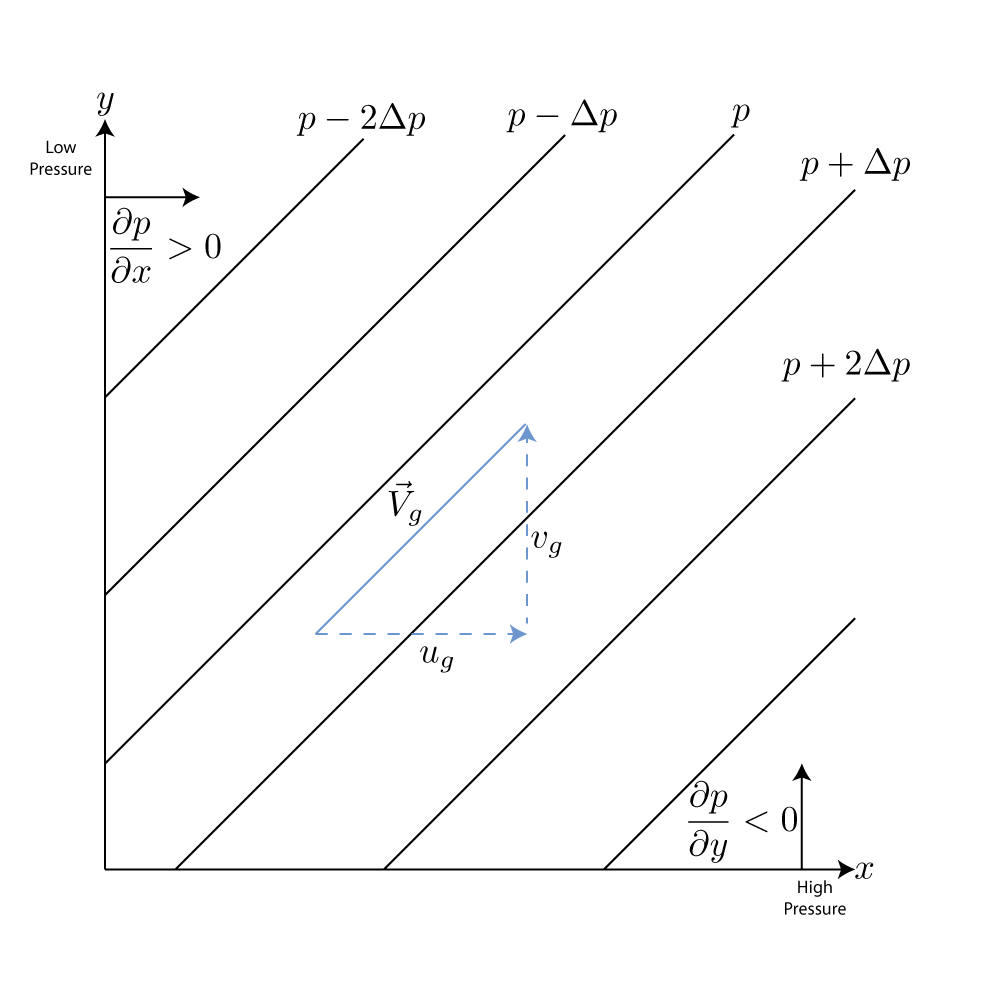
\includegraphics[width=0.7\textwidth]{fig1}	
	\end{figure}
\end{itemize}
\end{frame}
%------------------------------------------------
\begin{frame}{Geostrophic Approximation}
\begin{itemize}
	\item If we want to develop a prognostic equation using the geostrophic approximation, we must retain the acceleration term
	\begin{align*}
	\frac{Du}{Dt} &= fv - \frac{1}{\rho}\frac{\partial p}{\partial x}\\
	\frac{Dv}{Dt} &= -fu -\frac{1}{\rho}\frac{\partial p}{\partial y}
	\end{align*}
	Recall that 
	$$u_g = -\frac{1}{f\rho}\frac{\partial p}{\partial y}\qquad v_g = \frac{1}{f\rho}\frac{\partial p}{\partial x}$$
	Substitution yields
	\begin{align*}
	\frac{Du}{Dt} &= f(v-v_g)\\
	\frac{Dv}{Dt} &= -f(u-u_g)
	\end{align*}
	\item In other words, accelerations are proportional to the departure of the wind from the geostrophic wind
\end{itemize}
\end{frame}

%------------------------------------------------
\begin{frame}{Geostrophic Approximation}
$$\frac{Du}{Dt} = f(v-v_g) \qquad \frac{Dv}{Dt} = -f(u-u_g)$$
\begin{itemize}
	\item If you recall from scale analysis, the acceleration terms are an order of magnitude smaller than the Coriolis and pressure terms
	\item While geostrophic balance is a useful diagnosis tool, its application to weather forecasting is fraught with difficulty
	\item Why? The acceleration (very important to get right) is equal to the small difference between two large terms - which means it is susceptible to measurement errors in velocity or pressure gradient
\end{itemize}
\end{frame}

%------------------------------------------------
\begin{frame}{Geostrophic Approximation}
\begin{itemize}
	\item A useful comparison of the magnitude of the acceleration with the Coriolis force is through the ratio of their respective characteristic scales
	$$\frac{U^2/L}{f_oL}$$
	\item This non-dimensional number is called the \textit{Rossby NUmber}
	$$\mathrm{Ro} \equiv \frac{U}{f_oL}$$
	\item Named after Swedish meteorologist Carl-Gustav Rossby
	\item As Ro becomes smaller, rotational effects are more important and the geostrophic approximation is more valid
	\item Ro breaks down near the equator, where $f\rightarrow0$
\end{itemize}
\end{frame}
%------------------------------------------------
\subsection{Hydrostatic Approximation}
%------------------------------------------------
\begin{frame}{Hydrostatic Approximation}

\begin{itemize}
	\item Next, we examined large (synoptic) scales and applied scale analysis to the vertical component
	\begin{align*}
	\frac{Dw}{Dt} &= -\frac{1}{\rho}	\frac{\partial p}{\partial z} + 2\Omega u \cos \phi + \nu \vec \nabla^2 w + g_z\\
	\end{align*}
	\item We assumed mid-latitude, steady-state, and neglected non-linear terms and frictional effects
	\item Assumed $U\gg W$ and aligned gravity with $\khat$
\end{itemize}
\end{frame}
%------------------------------------------------
\begin{frame}{Hydrostatic Approximation}

\begin{itemize}
	\item The resulting expression is a balance between the vertical pressure gradient and gravity
	\item This balance is called the \textit{hydrostatic approximation}
	$$\frac{\partial p}{\partial z} = -\rho g$$
	\item This expression can be related to the hypsometric equation (see Lecture 5)
	\item In other words, vertical accelerations are small compared to gravity at large scales and so the pressure at any point is equal to the weight of the overlying air
\end{itemize}
\end{frame}
%------------------------------------------------
\subsection{Boussinesq Approximation}
%------------------------------------------------
\begin{frame}{Boussinesq Approximation}

\begin{itemize}
	\item This is really 3 assumptions motivated byt he fact that compressibility effects are often small for atmospheric flows	
	\begin{enumerate}
		\item Assume flow is incompressible: $\vec{\nabla} \cdot \vec U = 0$
		\item Material properties (viscosity, thermal diffusivity, and specific heat) are assumed constant
		\item  Density is allowed to vary in gravity term but not in inertia term
	\end{enumerate}
	\item Let's look at assumption 3
\end{itemize}
\end{frame}
%------------------------------------------------
\begin{frame}{Boussinesq Approximation}

\begin{itemize}
	\item In reality, $\rho$ may vary in ($x$, $y$, $z$, $t$)
	\item We want to approximate it based on the smallness of its deviation from the mean
	\item Define a base-state pressure based on constant density $\rho_0$ (i.e., reference atmosphere has constant density)
	$$\rho = \rho_0 + \rho^\prime$$
	Then
	$$p = \bar p + p^\prime$$
	where $\bar p$ is the solutions of $\partial \bar p / \partial z = -\rho_0 g$
\end{itemize}
\end{frame}
%------------------------------------------------
\begin{frame}{Boussinesq Approximation}

\begin{itemize}
	\item The equations of motion become
	$$(\rho_0 + \rho^\prime)\frac{D\vec U}{Dt} = -\vec{\nabla}  p^\prime \underbrace{- \vec{\nabla} \bar p - \rho_0 g \khat}_{\text{These cancel}} - \rho^\prime g \khat + \mu \vec{\nabla}^2 \vec{U}$$
	divide by $\rho_0$
	$$\left( 1 + \frac{\rho^\prime}{\rho_0}\right)\frac{D\vec U}{Dt} =  -\frac{1}{\rho_0}\vec{\nabla}  p^\prime - \frac{\rho^\prime}{\rho_0}g\khat + \nu \vec{\nabla}\vec{U}$$
	Assume $\rho^\prime/\rho_0 \ll 1$, so finally
	$$\frac{D\vec U}{Dt} = -\frac{1}{\rho_0}\vec{\nabla}  p^\prime - \frac{\rho^\prime}{\rho_0}g\khat + \nu \vec{\nabla}\vec{U}$$
\end{itemize}
\end{frame}
%------------------------------------------------
\begin{frame}{Boussinesq Approximation}

\begin{itemize}
	\item Now let's consider the term $\rho^{'}/\rho$. The equation of state is given by $p=\rho R T$, which is decomposed as
	$$\cfrac{\overline p}{R} +\cfrac{p^{'}}{R} = \overline{\rho}\ \overline{T} + \overline{\rho} T^{'} + \rho^{'}\overline{T} + \rho^{'}T^{'} $$
	Next, we apply Reynolds averaging
$$\overline{\cfrac{\overline p}{R}} + \overline{\cfrac{p^{'}}{R}} = \overline{\overline{\rho}\ \overline{T}} + \overline{\overline{\rho} T^{'}} + \overline{\rho^{'}\overline{T}} + \overline{\rho^{'}T^{'}} \longrightarrow \cfrac{\overline{p}}{R} = \overline{\rho}\ \overline{T}  +  \overline{\rho^{'}T^{'}} \rightarrow \cfrac{\overline{p}}{R} = \overline{\rho}\ \overline{T}$$
	\item Thus, the equation of state holds in the mean. This is reasonable because the equation of state was originally formulated from measurements made with crude, slow-response sensors. These sensors were essentially measuring mean quantities.
\end{itemize}
\end{frame}
%------------------------------------------------
\begin{frame}{Boussinesq Approximation}

\begin{itemize}
	\item Now let's subtract the mean equation of state from the full linearized form
	$$
\cfrac{\overline{p}}{R} +\cfrac{p^{'}}{R} - \cfrac{\overline{p}}{R} = \overline{\rho}\ \overline{T} + \overline{\rho} T^{'} + \rho^{'}\overline{T} + \rho^{'}T^{'} - \overline{\rho}\ \overline{T} \longrightarrow \cfrac{p^{'}}{R} = \overline{\rho} T^{'} + \rho^{'}\overline{T} + \rho^{'}T^{'}.$$
	\item Finally divide by the mean equation of state
	$$
\cfrac{p^{'}}{R} \cfrac{R}{\overline{p}} = \cfrac{\overline{\rho}}{\overline{\rho}} \cfrac{T^{'}}{\overline{T}} + \cfrac{\rho^{'}}{\overline{\rho}} \cfrac{\overline{T}}{\overline{T}} + \cfrac{\rho^{'}}{\overline{\rho}} \cfrac{T^{'}}{\overline{T}} \longrightarrow \cfrac{p^{'}}{\overline{p}} = \cfrac{\rho^{'}}{\overline{\rho}} + \cfrac{T^{'}}{\overline{T}} + \cfrac{\rho^{'}}{\overline{\rho}} \cfrac{T^{'}}{\overline{T}}.
$$
\item The last term is much smaller than the others is safely neglected, which leads to 
$$
\cfrac{p^{'}}{\overline{p}} = \cfrac{\rho^{'}}{\overline{\rho}} + \cfrac{T^{'}}{\overline{T}} \mbox{ .}
$$
\end{itemize}
\end{frame}
%------------------------------------------------
\begin{frame}{Boussinesq Approximation}
$$
\cfrac{p^{'}}{\overline{p}} = \cfrac{\rho^{'}}{\overline{\rho}} + \cfrac{T^{'}}{\overline{T}} \mbox{ .}
$$
\begin{itemize}
	\item This is the linearized perturbation ideal gas law. Scale analysis shows that
	$p^{'}/\overline{p} \rightarrow 0.1\ \hecto\pascal / 1000\ \hecto\pascal = 10^{-4}$, while $T^{'} / \overline{T} \rightarrow 1\ \kelvin / 300\ \kelvin = 3.33\time10^{-3}$. Thus, we can neglect the pressure term, yielding
	$$\cfrac{\rho^{'}}{\overline{\rho}} \approx - \cfrac{T^{'}}{\overline{T}} $$
	\end{itemize}
\end{frame}
%------------------------------------------------
\begin{frame}{Boussinesq Approximation}

\begin{itemize}
	\item Recalling that $T^{'} = T - \overline{T}$ and making use of the Poisson equation,  one can write
\begin{align*}
\cfrac{T^{'}}{\overline{T}} &= \frac{\theta \left(\cfrac{p}{p_0}\right)^{\frac{R}{c_p}} - \overline{\theta} \left(\cfrac{\overline{p}}{p_0}\right)^{\frac{R}{c_p}}}{\overline{\theta} \left(\cfrac{\overline{p}}{p_0}\right)^{\frac{R}{c_p}}} = \frac{\theta \left(\cfrac{\overline{p} + p^{'}}{p_0}\right)^{\frac{R}{c_p}} - \overline{\theta} \left(\cfrac{\overline{p}}{p_0}\right)^{\frac{R}{c_p}}}{\overline{\theta} \left(\cfrac{\overline{p}}{p_0}\right)^{\frac{R}{c_p}}}\\& \approx \frac{\theta \left(\cfrac{\overline{p}}{p_0}\right)^{\frac{R}{c_p}} - \overline{\theta} \left(\cfrac{\overline{p}}{p_0}\right)^{\frac{R}{c_p}}}{\overline{\theta} \left(\cfrac{\overline{p}}{p_0}\right)^{\frac{R}{c_p}}} \approx \cfrac{\theta - \overline{\theta}}{\overline{\theta}}.
\end{align*}
	\end{itemize}
\end{frame}
%------------------------------------------------
\begin{frame}{Boussinesq Approximation}

\begin{itemize}
	\item Thus, one can use the approximation that 
$$
\boxed{\cfrac{\rho^{'}}{\overline{\rho}} \approx - \cfrac{T^{'}}{\overline{T}} \approx - \cfrac{\theta^{'}}{\overline{\theta}}}
$$
\item We can use this approximation, we can write the equations of motion in terms of buoyancy
$$\boxed{\frac{D\vec U}{Dt} = -\frac{1}{\rho_0}\vec{\nabla}  p^\prime + \beta \theta^\prime + \nu \vec{\nabla}\vec{U}}$$
where $\beta = g\khat / \overline{\theta}$ is the buoyancy parameter
	\end{itemize}
\end{frame}

%------------------------------ ------------------
\begin{frame}{Boussinesq Approximation}

\begin{itemize}
	\item We can rewrite this expression by noting that
	$$\frac{1}{\rho_0}\vec{\nabla}  p^\prime = \frac{1}{\rho_0}\vec{\nabla} p - \frac{1}{\rho_0}\vec{\nabla}  \bar p$$
	where $$\frac{1}{\rho_0}\vec{\nabla}  \bar p = -g\khat$$
	
	\item Combined, we can write the equations of motion as
	$$\boxed{\frac{D\vec U}{Dt} = \frac{1}{\rho_0}\vec{\nabla} p -g\khat+ \beta \theta^\prime + \nu \vec{\nabla}\vec{U}}$$
	\end{itemize}
\end{frame}
%------------------------------ ------------------
\begin{frame}{Boussinesq Approximation}
$$\boxed{\frac{D\vec U}{Dt} = \frac{1}{\rho_0}\vec{\nabla} p -g\khat+ \beta \theta^\prime + \nu \vec{\nabla}\vec{U}}$$
\begin{itemize}
	\item The Boussinesq approximation essentially describes the residual between the pressure gradient force and the buoyancy force
	\item This is why we estimate in terms of deviations/perturbation from the hydrostatically-balanced base state
	\end{itemize}
\end{frame}

%------------------------------------------------
\end{document}

